\subsection{需求背景}
在车站接人、校园接送等场景中，固定上车点可能增加司机绕行与等候时间。如果乘客能够步行、骑行或乘公共交通移动一段距离，双方可能在其他地点更早会合。会合助手将双方的时间与乘客移动负担纳入同一次规划。
\subsection{位置输入与出行偏好}
用户通过搜索或地图选点设置双方位置，再选择乘客可用方式、步行上限，以及综合最优或地铁优先策略。用户也可向智能助手输入“我可以骑车”“尽量少走路”等要求，由助手理解偏好并调用规划功能。
\begin{figure}[H]\centering
\shot{preferences.png}{规划设置}{出行方式、计算策略与步行上限。}\hfill
\shot{chat.png}{智能助手入口}{通过自然语言补充出行要求。}
\caption{结构化偏好设置与自然语言输入入口}
\end{figure}
\clearpage
\noindent\begin{minipage}[t]{0.48\linewidth}\vspace{0pt}
\subsection{会合方案比较}
\begin{minipage}[t][4.8cm][t]{\linewidth}
结果页保留原地等待方案，并列出可行的移动会合方式。每个方案显示会合位置、预计会合用时和司机节省时间，地图展示双方路线。

图~\ref{fig:comparison} 的西安示例中，原地等待预计为 80 分钟；推荐方案的司机用时为 35 分钟，乘客为 42 分钟，预计会合用时为 42 分钟，比原地等待减少 38 分钟。
\end{minipage}
\par\centering
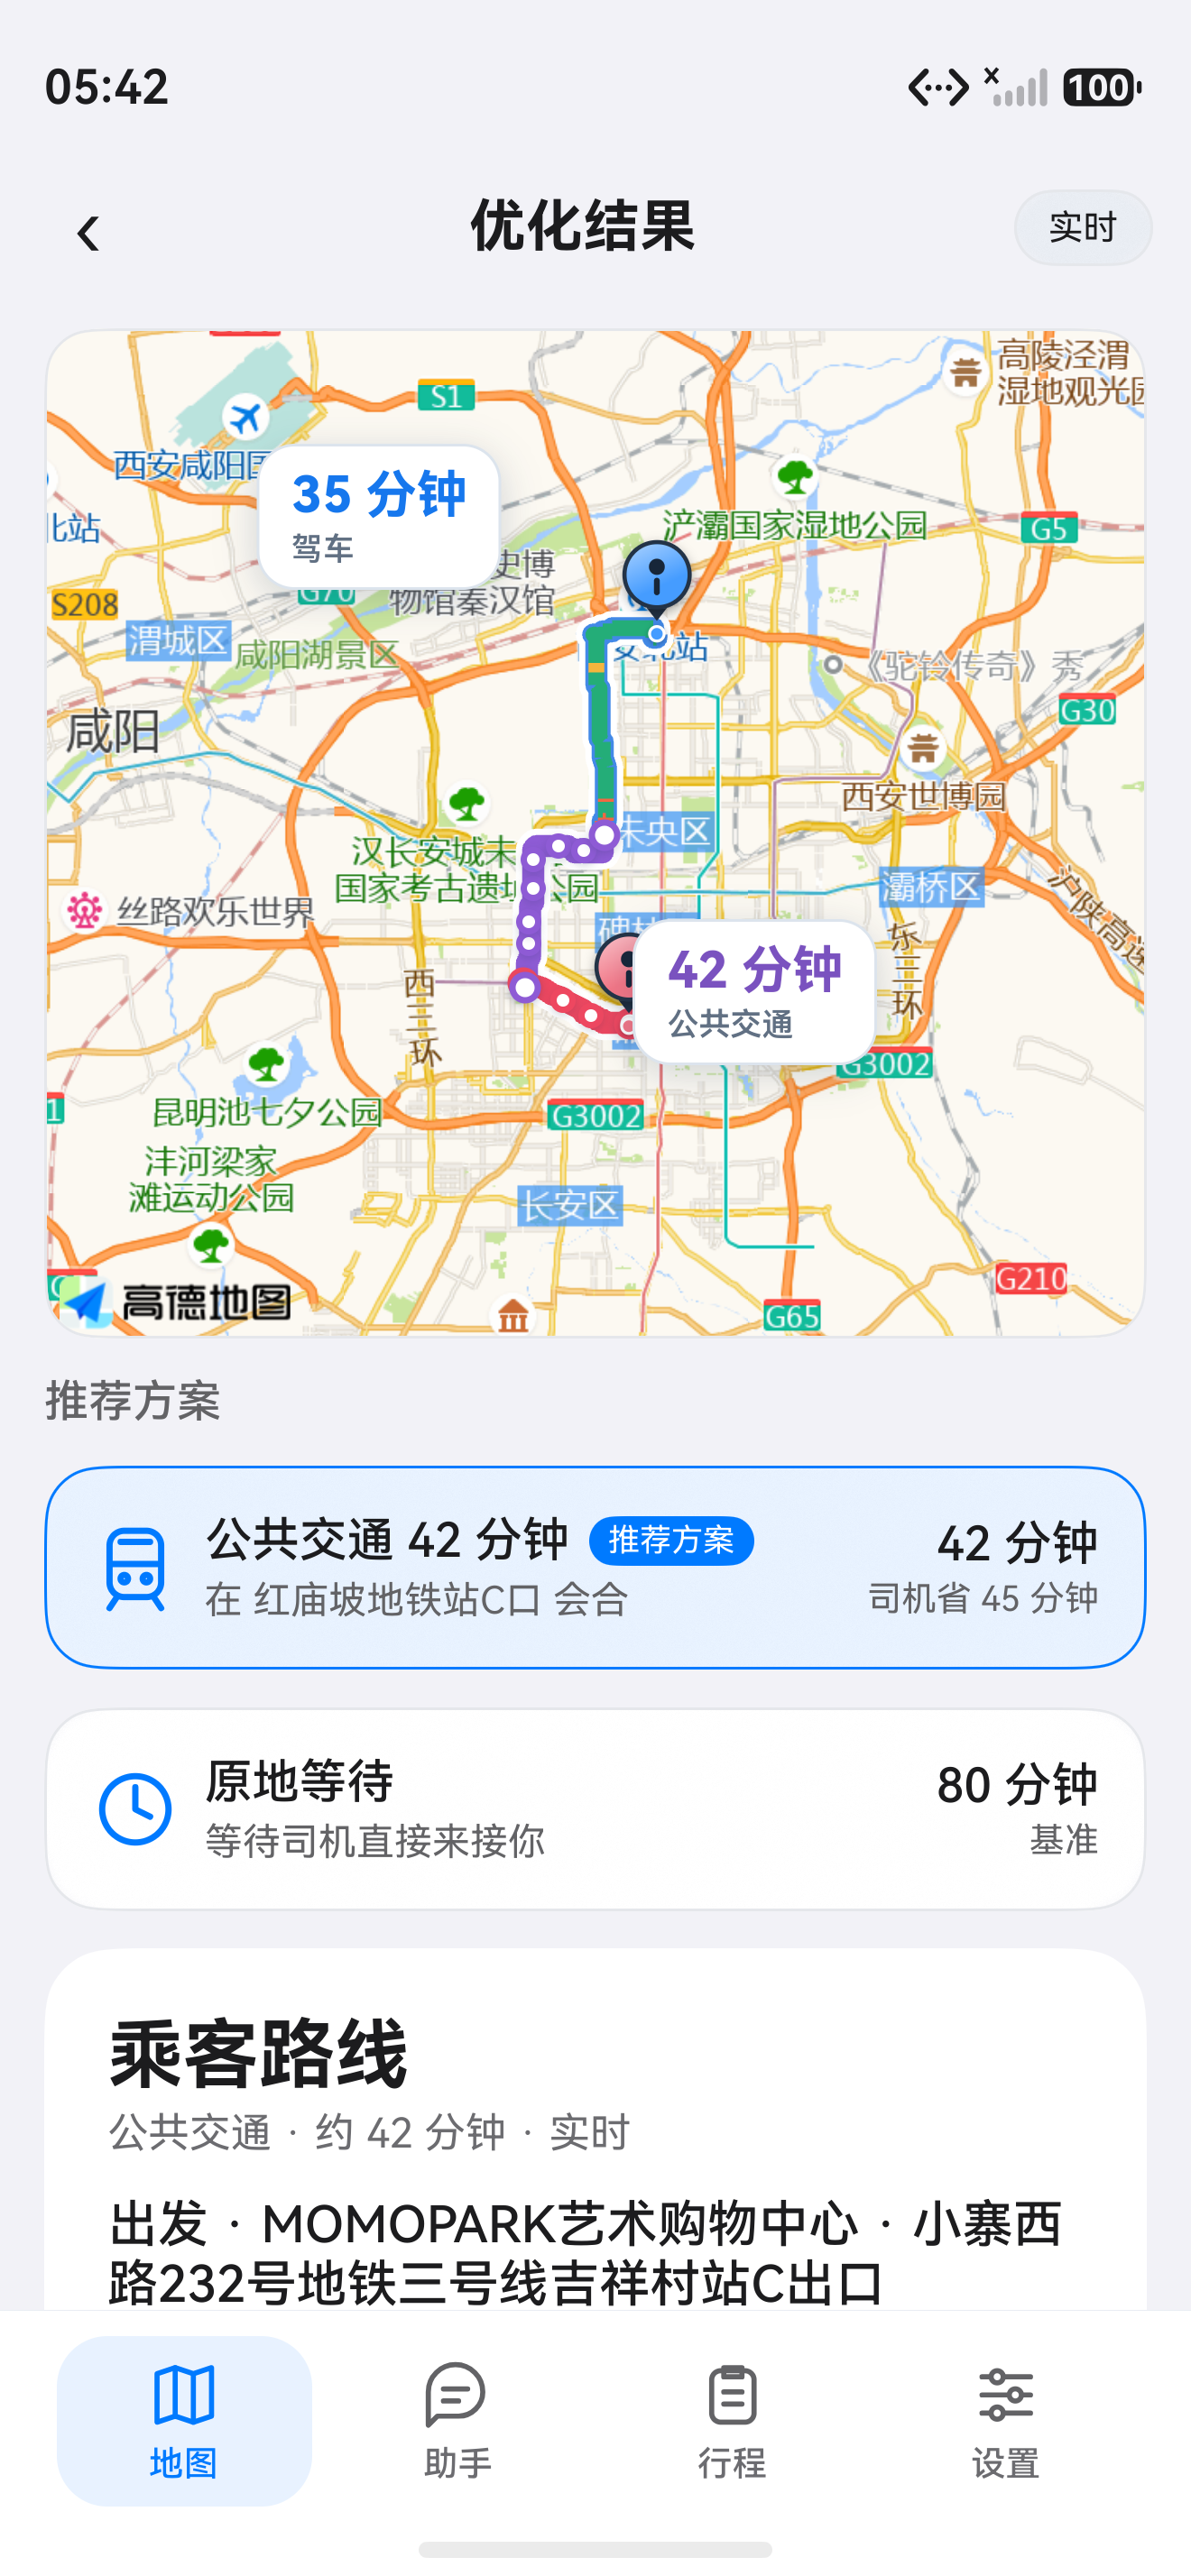
\includegraphics[height=12.8cm,width=\linewidth,keepaspectratio]{assets/plan.png}
\captionof{figure}{会合方案与双方路线比较}\label{fig:comparison}
\end{minipage}\hfill
\begin{minipage}[t]{0.48\linewidth}\vspace{0pt}
\subsection{公共交通路线详情}
\begin{minipage}[t][4.8cm][t]{\linewidth}
选择公共交通选项卡后，可查看乘客的具体路线。地图用不同颜色区分交通线路，页面下方按顺序列出地铁、步行与换乘步骤。

图~\ref{fig:transit} 展示了同一方案的分段行程，包括地铁 3 号线与 8 号线、上下车站、步行距离、预计用时和进出站口，便于乘客判断换乘与步行安排。
\end{minipage}
\par\centering
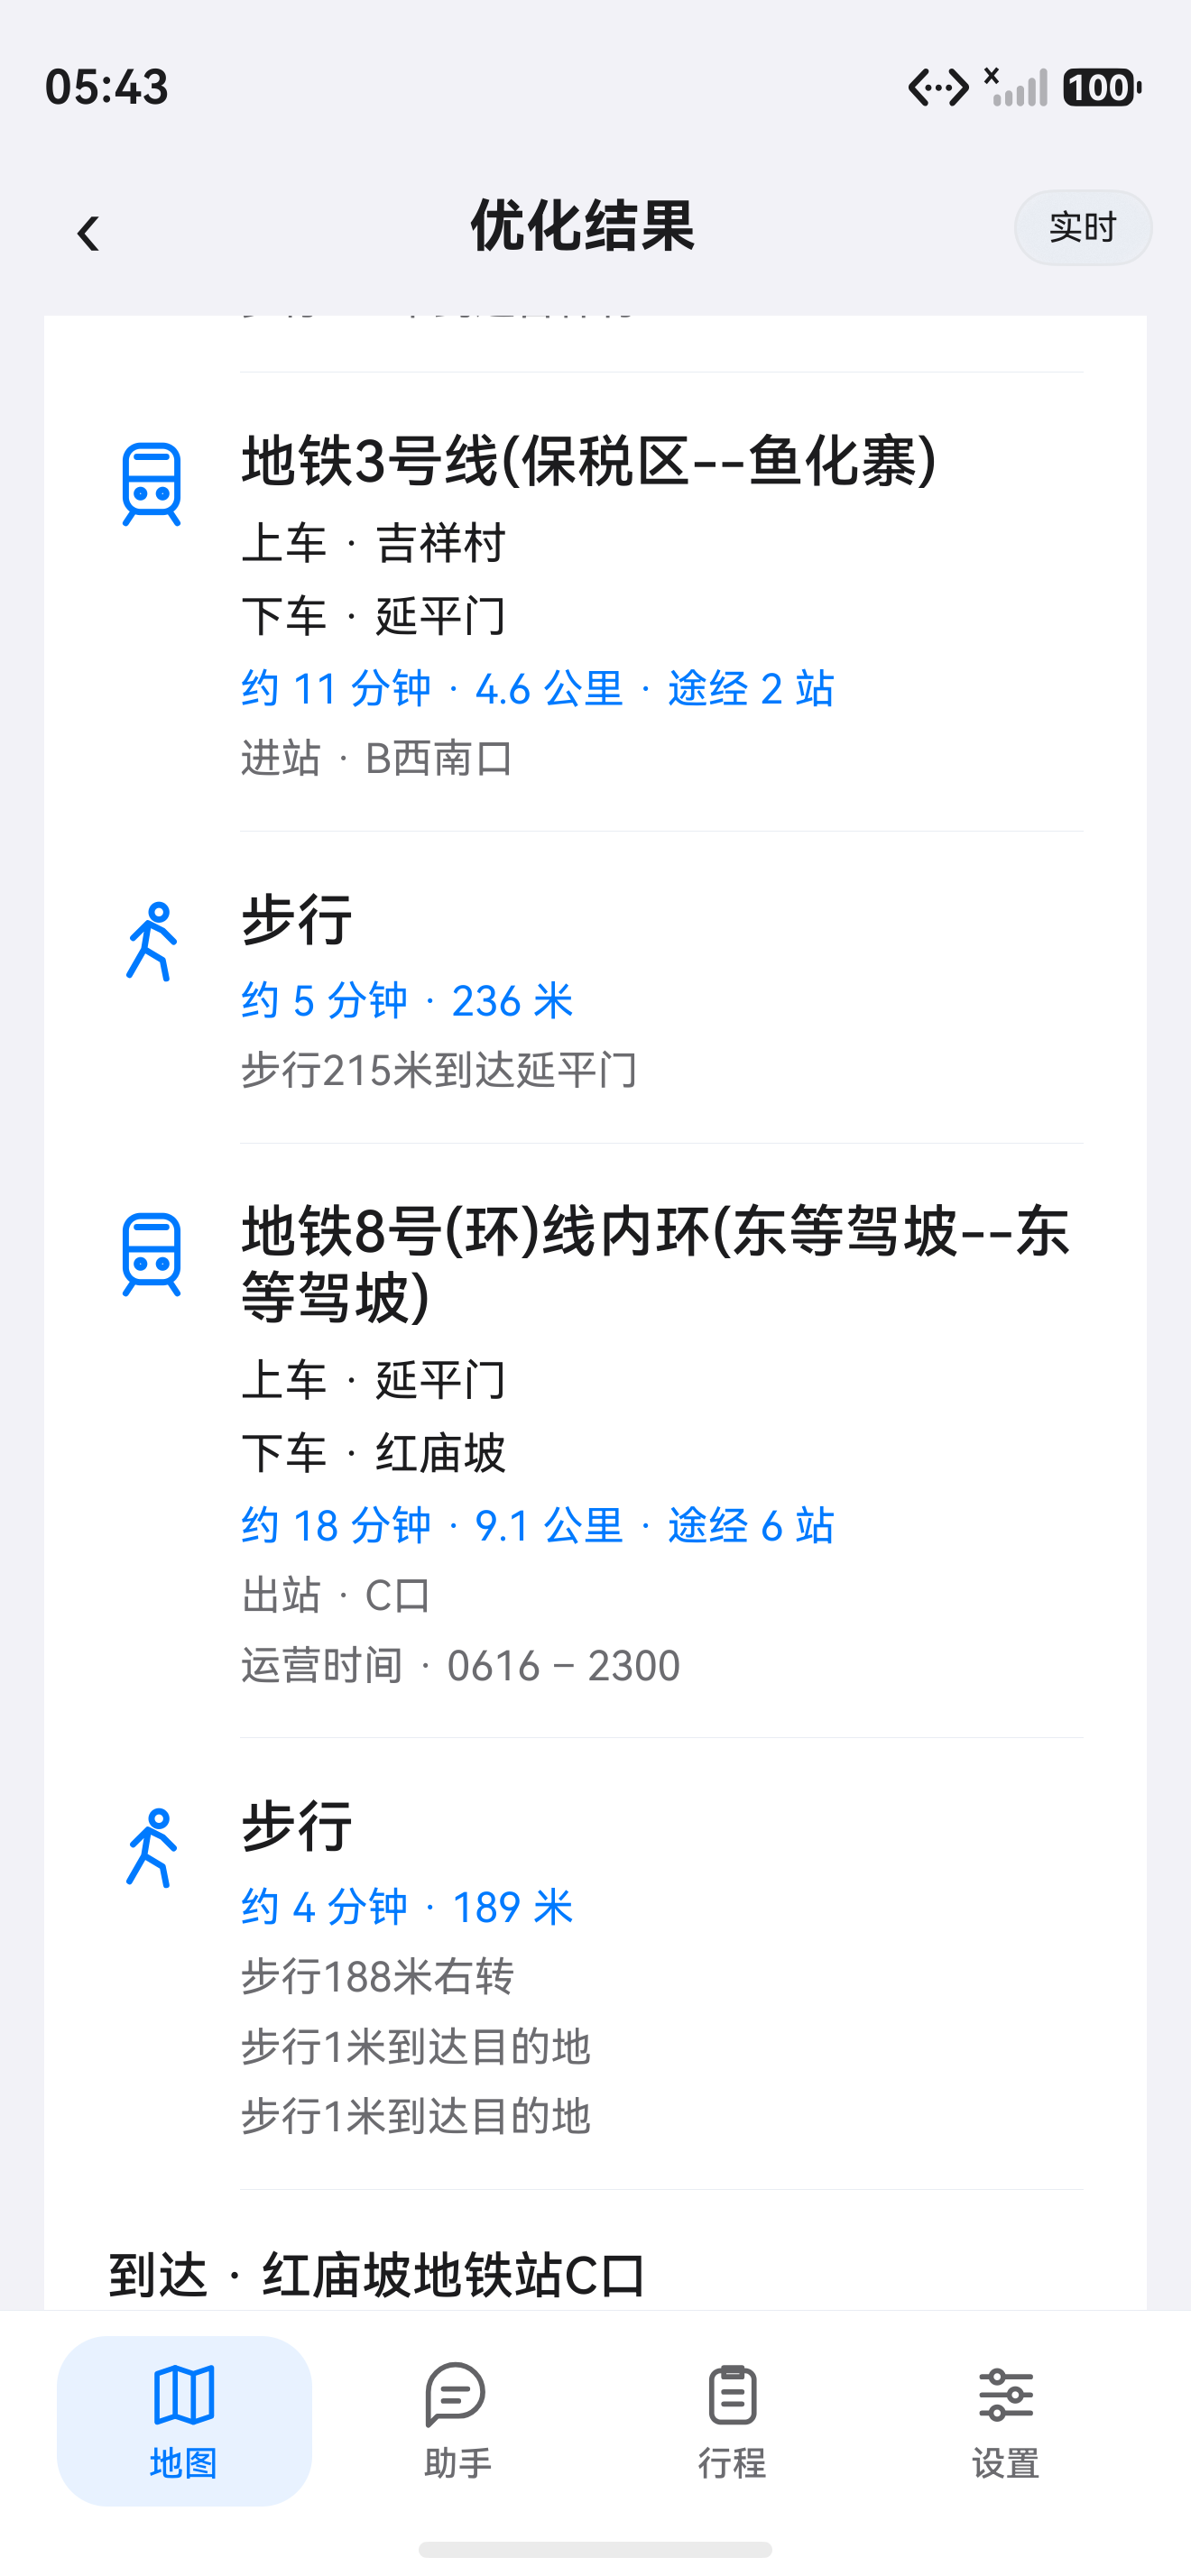
\includegraphics[height=12.8cm,width=\linewidth,keepaspectratio]{assets/passenger-route.png}
\captionof{figure}{公共交通方案的乘客分段行程}\label{fig:transit}
\end{minipage}
\par\vspace{12pt}
图~\ref{fig:comparison}、图~\ref{fig:transit} 为同一次模拟器运行的应用截图，数值为该次路线规划的预计结果。
\clearpage
\subsection{方案确认、分享与导航}
用户确认后，会合地点与路线保存在行程页，不会自动改变；调整地点时需主动重新规划。行程信息可复制分享给对方，并衔接地图导航。一部手机即可完成规划，对方通过分享内容了解会合安排。
\begin{figure}[H]\centering
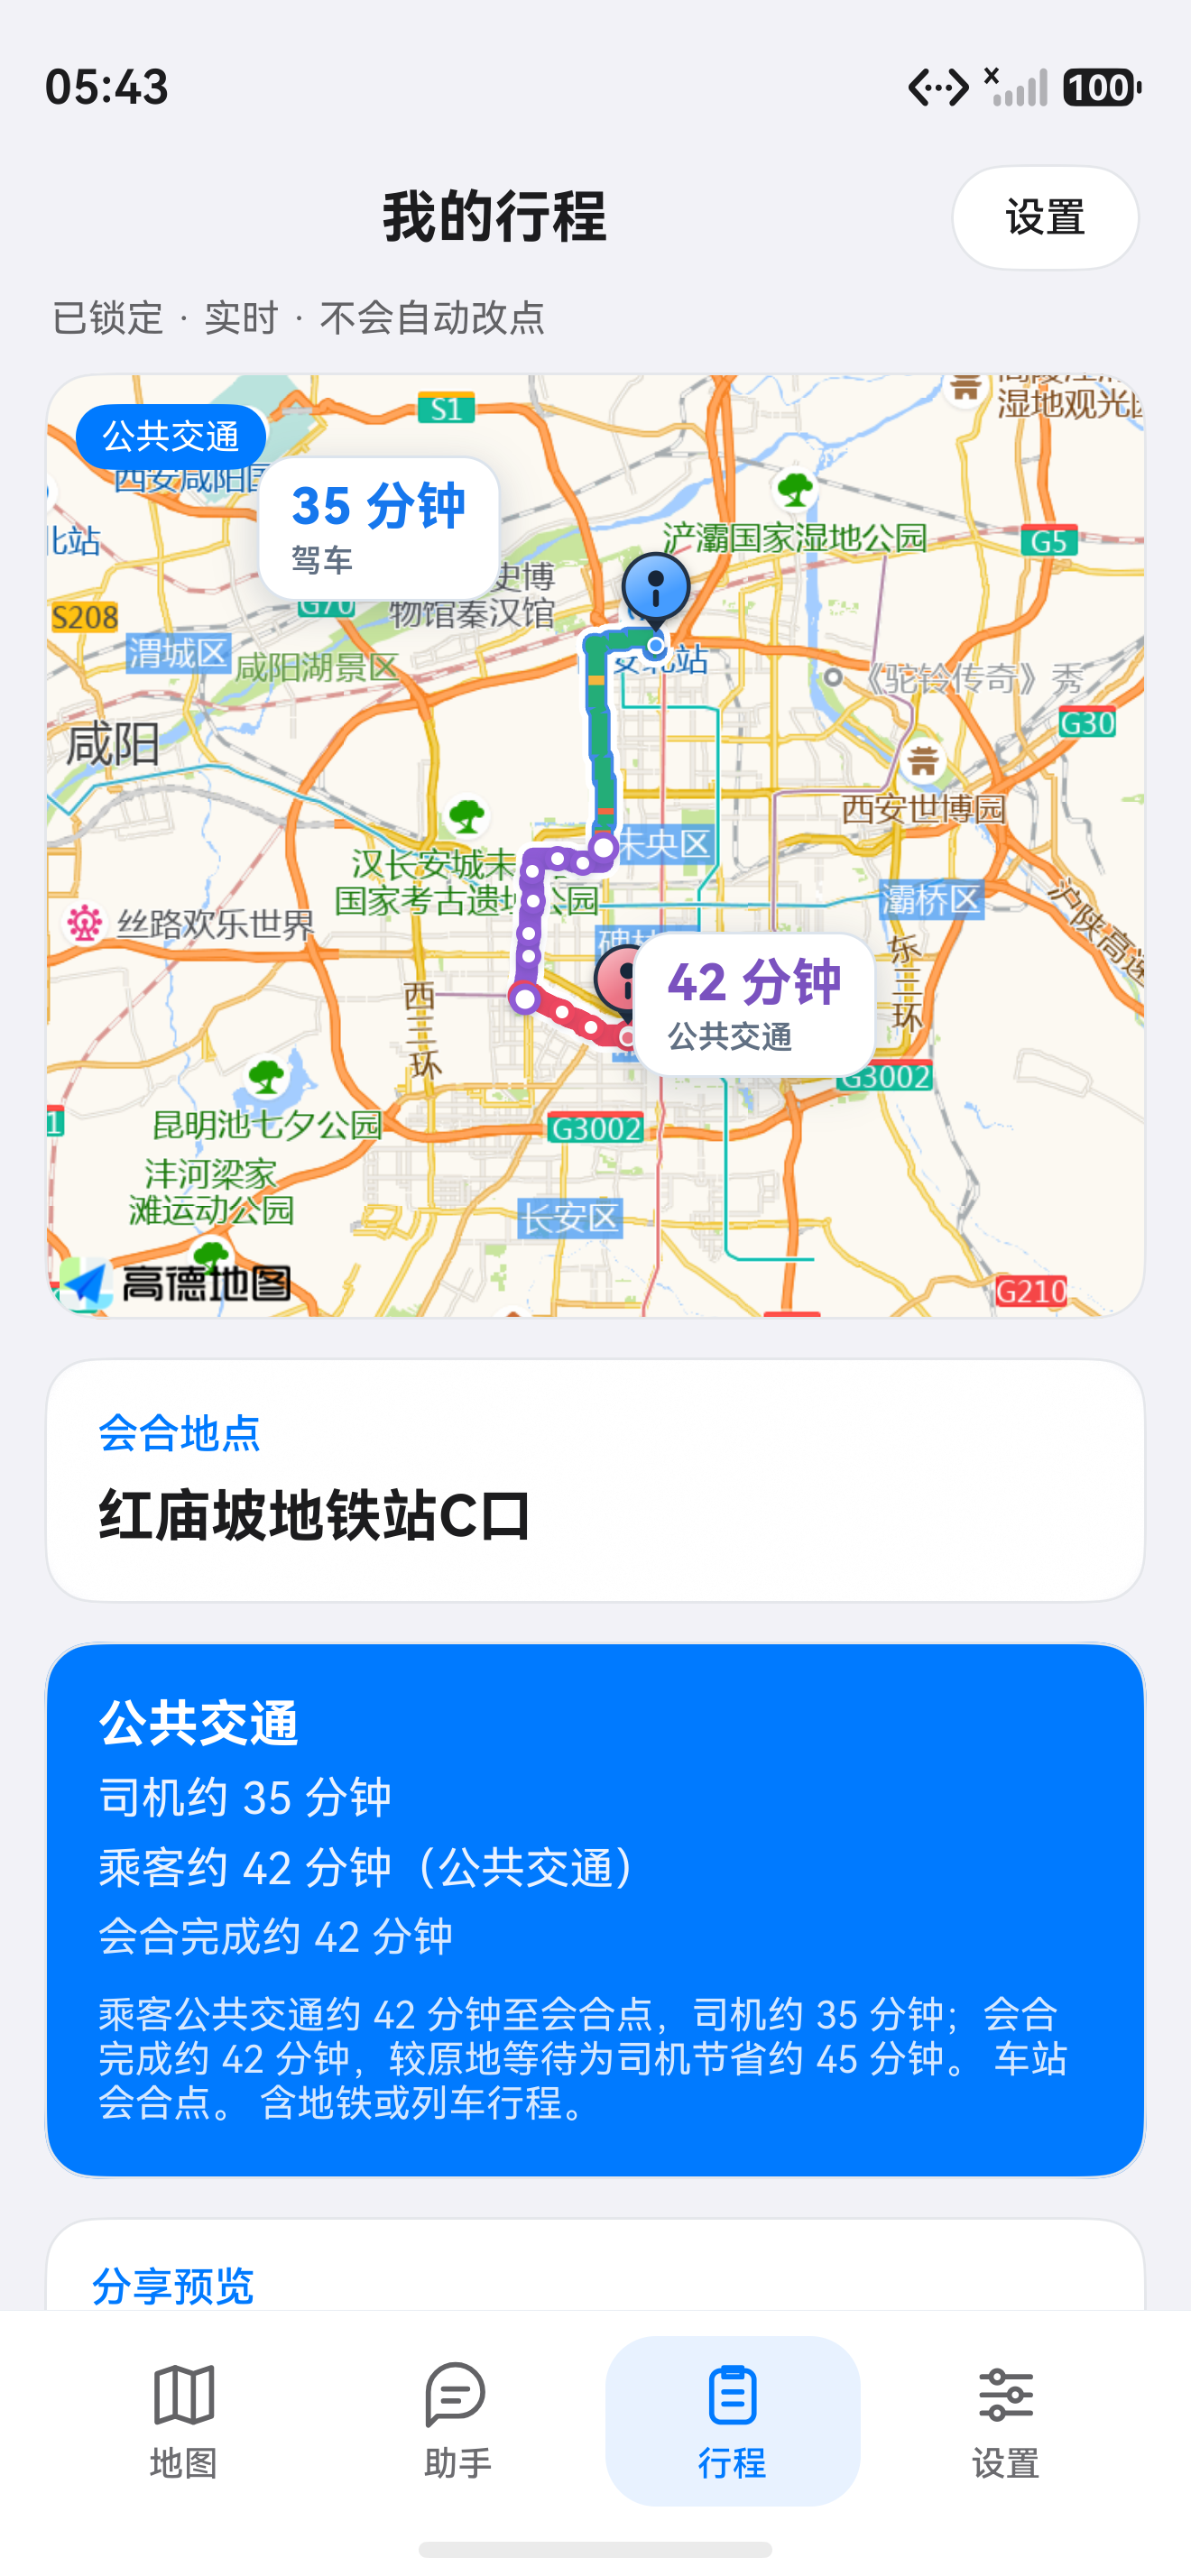
\includegraphics[height=12.5cm]{assets/locked.png}
\caption{确认后的行程页：会合地点、双方用时及路线}
\end{figure}
\subsection{功能实现}
应用采用 HarmonyOS 原生界面。地图服务提供路线和预计用时，本地规划引擎比较候选地点、双方到达时间及乘客移动负担；AI 负责理解偏好、调用工具和解释方案。没有足够改善时，应用推荐原地等待。普通规划可独立于 AI 服务使用。
\clearpage
\subsection{应用场景与发展前景}
会合助手适用于一方驾车、另一方具有短途移动条件的接送需求。其价值主要体现在：比较不同会合位置，减少单独查路线和协商地点的操作，并为乘客提供明确的到达步骤。
\begin{table}[H]\centering\caption{主要应用场景与对应需求}
\renewcommand{\arraystretch}{1.4}
\begin{tabularx}{\linewidth}{L{2.6cm}X}\toprule
\textbf{应用场景} & \textbf{对应需求}\\\midrule
亲友接送 & 结合司机路线和乘客出行意愿，提前确定双方可接受的会合地点。\\
校园与园区 & 比较不同出入口及周边位置，衔接司机驾车与乘客步行、骑行路线。\\
交通枢纽接送 & 利用车站周边公共交通，比较站外或沿途会合与直接到站接人的时间。\\
活动散场接送 & 在接送前比较周边候选位置，明确双方路线，减少临时寻找对方的沟通。\\\bottomrule
\end{tabularx}
\end{table}

后续可进行多机同步功能的开发，实时显示双方当前位置。或根据当前路况的变化选择推荐更优的会合点，以及加强校园接送场景的优化，精确到出入口等等。